%%%%%%%%%%%%%%%%%%%%%%%%%%%%%%%%%%%%%%%%%%%%%%%%%%%%%%%%%%%%%%%%%%%%%%%%%%%%%%%%%%
\begin{frame}[fragile]\frametitle{}
\begin{center}
{\Large PyTorch Geometric}
\end{center}
\end{frame}


%%%%%%%%%%%%%%%%%%%%%%%%%%%%%%%%%%%%%%%%%%%%%%%%%%%%%%%%%%%
\begin{frame}[fragile]\frametitle{What is Pytorch Geometric (PyG)?}

\begin{itemize}
\item A python framework for deep learning on irregular structures like graphs, point clouds and manifolds, a.k.a Geometric Deep Learning 
\item Contains relational learning and 3D data processing methods such as Graph Neural Network(GNN)
\item Developed by Matthias Fey, eJan Eric Lenssn from TU Dortmund University. 
\item Functionalities provided:
	\begin{itemize}
	\item Neighbourhood Aggregation
	\item Global Pooling
	\item Hierarchical Pooling
	\item Mini-Batch Handling
	\item Processing of Datasets
	\end{itemize}
\end{itemize}

\end{frame}

%%%%%%%%%%%%%%%%%%%%%%%%%%%%%%%%%%%%%%%%%%%%%%%%%%%%%%%%%%%
\begin{frame}[fragile]\frametitle{Installation}

\begin{itemize}
\item Install PyTorch $>= 1.4.0$ via, say, \lstinline|conda install pytorch torchvision torchaudio cpuonly -c pytorch|
\item Note down Pytorch version: \lstinline|python -c "import torch; print(torch.__version__)"|
\item Note down CUDA version: \lstinline|python -c "import torch; print(torch.version.cuda)"|
\item Install dependencies (Replace TORCH with the PyTorch version and CUDA with the CUDA version, below)
\item Install PyG \lstinline|pip install torch-geometric|
\end{itemize}

\begin{lstlisting}
pip install torch-scatter -f https://pytorch-geometric.com/whl/torch-${TORCH}+${CUDA}.html
pip install torch-sparse -f https://pytorch-geometric.com/whl/torch-${TORCH}+${CUDA}.html
pip install torch-cluster -f https://pytorch-geometric.com/whl/torch-${TORCH}+${CUDA}.html
pip install torch-spline-conv -f https://pytorch-geometric.com/whl/torch-${TORCH}+${CUDA}.html 
\end{lstlisting}

\end{frame}

%%%%%%%%%%%%%%%%%%%%%%%%%%%%%%%%%%%%%%%%%%%%%%%%%%%%%%%%%%%
\begin{frame}[fragile]\frametitle{Representation}

Creating an unweighted and undirected graph with three nodes and four edges. 

\begin{center}
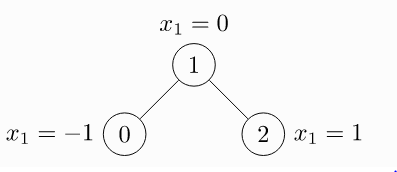
\includegraphics[width=0.3\linewidth,keepaspectratio]{pyg1}
\end{center}	  


\begin{lstlisting}
import torch
from torch_geometric.data import Data
edge_index = torch.tensor([[0, 1, 1, 2],
                            [1, 0, 2, 1]], dtype=torch.long)
x = torch.tensor([[-1], [0], [1]], dtype=torch.float)
data = Data(x=x, edge_index=edge_index) 
\end{lstlisting}

\end{frame}

%%%%%%%%%%%%%%%%%%%%%%%%%%%%%%%%%%%%%%%%%%%%%%%%%%%%%%%%%%%
\begin{frame}[fragile]\frametitle{Datasets}

PyG contains many benchmark datasets e.g., : all Planetoid datasets (Cora, Citeseer, Pubmed), all graph classification datasets from http://graphkernels.cs.tu-dortmund.de and their cleaned versions, etc


\begin{lstlisting}
from torch_geometric.datasets import TUDataset
dataset = TUDataset(root='/tmp/ENZYMES', name='ENZYMES')
\end{lstlisting}

\end{frame}

%%%%%%%%%%%%%%%%%%%%%%%%%%%%%%%%%%%%%%%%%%%%%%%%%%%%%%%%%%%
\begin{frame}[fragile]\frametitle{Data-loader}

PyG provides \lstinline|torch_geometric.data.DataLoader| for merging the data objects to a mini batch.

\begin{lstlisting}
from torch_geometric.datasets import TUDataset
from torch_geometric.data import DataLoader
dataset = TUDataset(root='/tmp/ENZYMES', name='ENZYMES', use_node_attr=True)
loader = DataLoader(dataset, batch_size=32, shuffle=True)
for batch in loader:
	 print(batch)
	 print(batch.num_graphs)
\end{lstlisting}

\end{frame}

%%%%%%%%%%%%%%%%%%%%%%%%%%%%%%%%%%%%%%%%%%%%%%%%%%%%%%%%%%%
\begin{frame}[fragile]\frametitle{Data-Transform}

PyG provides its data transformation utility whose input is Data object and output is transformed Data object.

\begin{lstlisting}
import torch_geometric.transforms as T
from torch_geometric.datasets import ShapeNet
dataset = ShapeNet(root='/tmp/ShapeNet', categories=['Airplane'],
									 pre_transform=T.KNNGraph(k=6))
dataset[0] 
\end{lstlisting}

\end{frame}

%%%%%%%%%%%%%%%%%%%%%%%%%%%%%%%%%%%%%%%%%%%%%%%%%%%%%%%%%%%
\begin{frame}[fragile]\frametitle{Graph Neural Network Definition}

Create a two-layer GCN network.

\begin{lstlisting}
import torch
import torch.nn.functional as F
from torch_geometric.nn import GCNConv
class Net(torch.nn.Module):
	 def __init__(self):
			 super(Net, self).__init__()
			 self.conv1 = GCNConv(dataset.num_node_features, 16)
			 self.conv2 = GCNConv(16, dataset.num_classes)
	 def forward(self, data):
			 x, edge_index = data.x, data.edge_index
			 x = self.conv1(x, edge_index)
			 x = F.relu(x)
			 x = F.dropout(x, training=self.training)
			 x = self.conv2(x, edge_index)
			 return F.log_softmax(x, dim=1) 
\end{lstlisting}

\end{frame}
%%%%%%%%%%%%%%%%%%%%%%%%%%%%%%%%%%%%%%%%%%%%%%%%%%%%%%%%%%%
\begin{frame}[fragile]\frametitle{Training and Evaluation}

Let’s train this model on the train nodes for 200 epochs.

\begin{lstlisting}
device = torch.device('cuda' if torch.cuda.is_available() else 'cpu')
model = Net().to(device)
data = dataset[0].to(device)
optimizer = torch.optim.Adam(model.parameters(), lr=0.01, weight_decay=5e-4)
model.train()
for epoch in range(200):
	 optimizer.zero_grad()
	 out = model(data)
	 loss = F.nll_loss(out[data.train_mask], data.y[data.train_mask])
	 loss.backward()
	 optimizer.step() 
	 
# Evaluate the model on test data.
model.eval()
_, pred = model(data).max(dim=1)
correct = int(pred[data.test_mask].eq(data.y[data.test_mask]).sum().item())
acc = correct / int(data.test_mask.sum())
print('Accuracy: {:.4f}'.format(acc)) 	 
\end{lstlisting}

\end{frame}
